\newpage
\section{Auswertung}
Die Werte der Bauteile des Schwingkreises sind:
\begin{align*}
    L&=\SI{16.78(09)}{\micro\henry}\\
    C&=\SI{2.066(006)}{\nano\farad}\\
    R_1&=\SI{67.2(2)}{\ohm}\\
    R_2&=\SI{682(1)}{\ohm}\\
\end{align*}
\subsection{Schwingungskurve}
\noindent
Aus der Schwingungskurve lässt sich mit Hilfe der Messwerte in der Tabelle \ref{tab:Uamp} eine einhüllende Funktion bestimmen. 
Dafür wird eine Fit-Funktion $U(t)$ bestimmt. Sie hat die Form:
\begin{equation}
    U(t)=A_0 \symup{e}^{-\mu t} \nonumber
\end{equation}
Über eine Ausgleichsrechnung mit den Beträgen der Werte von $U_\text{Amp}$, da die Kurve zur x-Achse symmetrisch ist,
bestimmen sich die Konstanten zu:
\begin{align*}
    A_0&=\SI{13.9205(2535)}{\V} & \mu&=(\num{1846.24473 \pm 58.380141 }) \mathrm{\frac{1}{s}} 
\end{align*}
Die Messwerte und der Fit ist in Abbildung \ref{img:huell} abgebildet.
\begin{figure}[H]
    \centering
    \includegraphics[width=0.7\textwidth]{build/plots/plot0.pdf}
    \caption{Die Messwerte der gedämppften Schwingung mit der einhüllenden Fit-Funktion.}
    \label{img:huell}
\end{figure}
\noindent
Mit diesen Werten lässt sich dann der der effektive Widerstand und die Abklingzeit des Schwingkreises bestimmen. 
Dafür werden die folgenden Gleichungen genutzt:
\begin{align*}
    R_\text{eff}&=\mu \cdot 4\pi L\\
    R_\text{eff}&= \SI{389.3060(124861)}{\ohm}  \\\\
    T_\text{ex}&=\frac{1}{2\pi\mu}\\
    T_\text{ex}&=\SI{86.2046838617(27258800232)}{\micro\second}
\end{align*}
Die Abweichung des genutzten Widerstandes von $R_\text{eff}$ beträgt:
\begin{equation}
    R_\text{eff}-R_1=\SI{322.1060(124877)}{\ohm}
\end{equation}
Eine Abweichung von $\SI{50}{\ohm}$ wäre zu erwarten gewesen, da dies der Innenwiderstands des Generators ist.
Die tatsächliche Abweichung von $\approx \SI{300}{\ohm}$ könnte sich über ein Problem mit dem Generator erklären, welches bei späteren Messungen 
aufgefallen ist. Da diese Messung noch mit dem \enquote*{defekten} Nadelimpulsgenerator durchgeführt wurde könnte er für die Abweichung verantwortlich sein.\\
Die nachfolgenden Rechnungen werden deshalb mit einem Widerstand von $R_1+\SI{50}{\ohm}$ durchgeführt.

\begin{table}[H]
    \centering
    \begin{tabular}{S [table-format=2.1] S [table-format=3.1]}
        \toprule
        {$U_\text{Amp} \mathbin{\scalebox{1.5} / }\si{\volt}$} & {$t_\text{Amp} \mathbin{\scalebox{1.5} / }\si{\micro\second}$}\\
        \midrule
        14.0 & 0.0 \\
        -11.5 & 14.0\\
        10.5 & 27.6\\
        -8.3 & 42.0\\
        7.8 & 54.00\\
        -6.0 & 68.0\\
        5.8 & 82.0\\
        -4.2 & 95.0\\
        4.1 & 108.0\\
        -3.0 & 122.0\\
        3.1 & 136.0\\
        -2.2 & 150.0\\
        2.5 & 163.0\\
        \bottomrule
    \end{tabular}
\caption{Die Messwerte der Amplitudenspannung mit ihren korrespondierenden Zeiten.}
\label{tab:Uamp}
\end{table}





\subsection{Aperiodischer Grenzfall}
\noindent
Die Messung zur Bestimmung des Widerstandes, bei dem der aperiodische Grenzfall eintritt, hat einen Wert von:
\begin{equation}
    R_\text{ap}=\SI[]{1925}[]{\ohm} \nonumber
\end{equation}
Der theoretische Wert und die relative Abweichung von ihm, im Bezug auf den Theoriewert, berechnet sich dann zu:
\begin{align*}
    R_\text{ap theo}&= \sqrt{\frac{4L}{C}}=\SI{5699.8157(923168)}{\ohm}\\
    \frac{R_\text{ap theo}-R_\text{ap}}{R_\text{ap theo}}&=\SI{66.22698(54700)}{\percent}
\end{align*}
Die Abweichung der Werte lässt sich durch die in der Rechnung nicht beachteten Widerstände der anderen Bauteile erklären. 
Allerdings kann damit keine Abweichung dieser Größe erklärt werden. Dafür kann also wieder der Generator verantwortlich gehalten werden.


\subsection{Resonanzüberhöhung}
Anschließend wird die Resonanzüberhöhumng untersucht. 
Die Messwerte der mit der angelegten Spannung normierten Kondensatorspannung und ihrerkorrespondierenden Frequenzen finden sich in Tabelle \ref{tab:Uu0}.
Aus diesen Messwerten lässt sich der theoretische Faktor für die Resonanzüberhöhung $q_\text{theo}$ bestimmen.
Die experimentelle Resonanzüberhöhung lässt sich durch ablesen des Maximums aus den Messwerten bestimmen. \\
Dies entspricht dem Wert $q_\text{exp}=3.8$.
$q_\text{theo}$ berechnet sich über die folgenden Gleichungen, wobei $R$ dem Gesamtdämpfungswiderstand entspricht.
\begin{align*}
    q_\text{theo}&= \frac{1}{\omega_0RC}& \omega_0&=\sqrt{\frac{1}{LC}}\\
    \implies q_\text{theo}&=\sqrt{\frac{L}{R^2C}}=\SI{24.3(4)}{}
\end{align*}
Dies führt zu einer relativen Abweichung des experimentellen vom theoretischen Wert von $\SI{84.37(25)}{\percent}$.
In der folgenden Abbildung sind die Messwerte halblogarithmisch aufgetragen.
\begin{figure}[H]
    \centering
    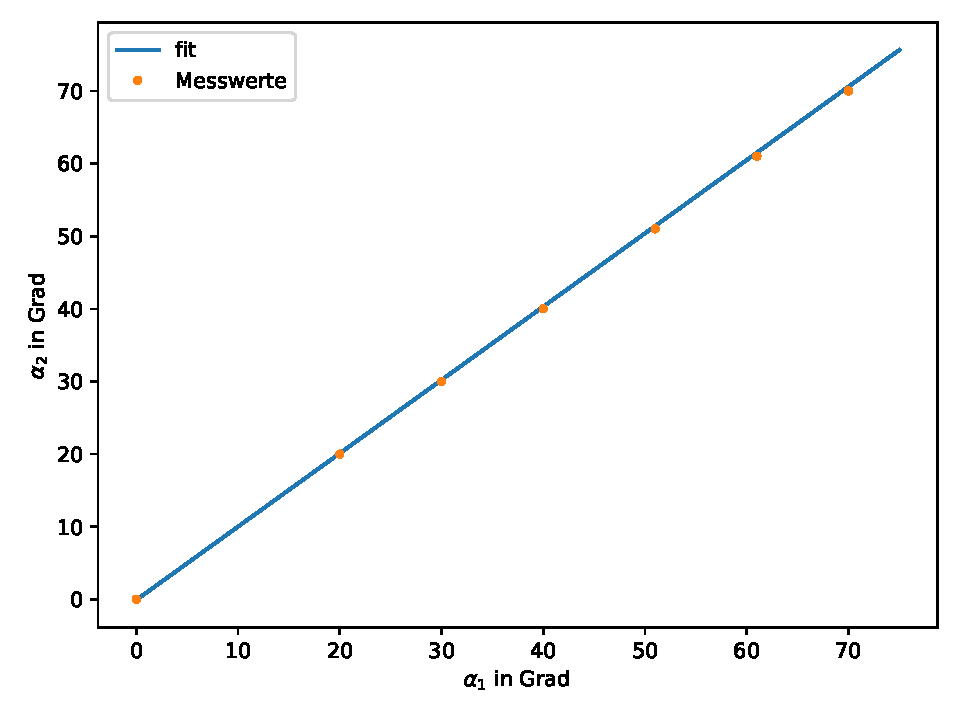
\includegraphics[width=0.7\textwidth]{build/plots/plot1.pdf}
    \caption{Die Messwerte zur Resonanzüberhöhung halblogarithmisch dargestellt.}
    \label{img:Uu0}
\end{figure}
\noindent
Für die Bestimmung der experimentellen Halbwertsbreite werden die Messwerte um den Peak mit einer quadratischen Funktion angenähert und der Schnittpunkt
mit ihr bei den Spannungswerten $\frac{U_\text{max}}{\sqrt{2}}$ bestimmt. Dies wird in der Abbildung \ref{img:Uu0halb} noch einmal veranschaulicht.
Dort sind die Messwerte des relevanten Wertebereiches linear dargestellt.
Außerdem sind die Schnittgerade bei $\frac{U_\text{max}}{\sqrt{2}}$ und die quadratische Fit-Funktion eingezeichnet.\\
Der Fit besitzt dabei die Form:
\begin{equation*}
    f(x)= A*x**2 +B*x+ C
\end{equation*}
mit 
\begin{table}[H]
    \centering
    \sisetup{table-format=1.3}
    \begin{tabular}{ S | S [table-format=2.5] @{$ \pm{}$} S [table-format=4.5]  }
        \toprule
        {Parameter} & \multicolumn{2}{c}{ Bestimmte Werte} \\
        \midrule
        \text{A}	& \num{-8.3}\SI{1e-8}{}& \num{0.5}\SI{1e-8}{} \\
        \text{B}	&\num{0.00432}  & \num{0.00028}  \\
        \text{C}	&\num{-52}  & \num{4}  \\
        \bottomrule
    \end{tabular}
\caption {Berechnete Werte für die quadratische Fit-Funktion gerundet auf die fünfte Nachkommastelle.}
\label{tab:signum}
\end{table}















\begin{table}[H]
    \centering
    \begin{tabular}{S [table-format=1.2] S [table-format=2.0]}
        \toprule
        {$\frac{U}{\symup{U_0}}$} & {$f \mathbin{\scalebox{1.5} / } \si{\kilo\hertz}$}\\
        \midrule
        1.08 & 5\\
        1.24 & 10\\
        1.44 & 15\\
        2.16 & 20\\
        2.40 & 21\\
        3.00 & 23\\
        3.40 & 24\\
        3.72 & 25\\
        3.80 & 26\\
        3.64 & 27\\
        3.12 & 28\\
        2.44 & 30\\
        1.60 & 33\\
        1.24 & 35\\
        0.84 & 40\\
        0.60 & 45\\
        0.44 & 50\\
        \bottomrule
    \end{tabular}
\caption{Die Messwerte Spannung im Verhältnis zur angelegten Spannung und die dazugehörigen Frequenzen.}
\label{tab:Uu0}
\end{table}

\begin{table}[H]
    \centering
    \begin{tabular}{S [table-format=2.1] S [table-format=2.1] S [table-format=1.3]}
        \toprule
        {$f \mathbin{\scalebox{1.5} / } \si{\kilo\hertz}$} & {$\increment t \mathbin{\scalebox{1.5} / } \si{\micro\second}$} & {$\phi \mathbin{\scalebox{1.5} / } \si{\radian}$}\\
        \midrule
        5.0& 0.0 & 0.000  \\
        10.0 & 1.0 & 0.063 \\
        12.0 & 1.5 & 0.113 \\
        14.0 & 1.5 & 0.132 \\
        20.0 & 0.0 & 0.000 \\
        25.0 & 0.5 & 0.079 \\
        30.0 & 1.0 & 0.188 \\
        35.0 & 1.5 & 0.330 \\
        35.7 & 3.0 & 0.674 \\
        36.2 & 4.0 & 0.911 \\
        36.7 & 6.0 & 1.385 \\
        37.5 & 8.0 & 1.885 \\
        38.0 & 10.0 & 2.388\\
        38.2 & 11.0 & 2.644\\
        38.7 & 11.0 & 2.678\\
        40.0 & 11.0 & 2.765\\
        42.5 & 11.5 & 3.071\\
        45.0 & 11.0 & 3.110\\
        \bottomrule
    \end{tabular}
\caption{Die Messwerte der Phasenverschiebung zwischen Kondensator- und Erregerspannung bei unterschiedlichen Frequenzen. $\increment t$ ist dabei die Zeitdifferenz zwishen zwei Amplituden und $\phi$ diese umgewandelt in einen Winkel.}
\label{tab:phi}
\end{table}





\begin{table}[H]
    \centering
    \sisetup{table-format=1.3}
    \begin{tabular}{ S | S [table-format=5.5] @{$ \pm{}$} S [table-format=2.5] S }
        \toprule
        {Parameter} & \multicolumn{3}{c}{ Bestimmte Werte} \\
        \midrule
        \text{A}	&\num{2.94167}  & \num{0.08634} & \; \si{\radian}\\
        \text{B}	&\num{36988.06355}  & \num{84.81132} & \\
        \text{C}	&\num{0.08872}  & \num{0.05578} & \; \si{\radian}\\
        \text{D}	&\num{838.78531}  & \num{67.35911} & \\
        \bottomrule
    \end{tabular}
\caption {Berechnete Werte für die Signums-Funktion gerundet auf die fünfte Nachkommastelle.}
\label{tab:signum}
\end{table}




\begin{table}[H]
    \centering
    \sisetup{table-format=1.3}
    \begin{tabular}{ S | S [table-format=2.2] @{$ \quad \pm{}$} S [table-format=1.2] S [table-format=2.2]  S [table-format=2.2] @{$ \quad \pm{}$} S [table-format=1.2] }
        \toprule
        \multicolumn{1}{c|}{Frequenz} & \multicolumn{2}{p{4cm}}{\centering Theoretischer Wert \\$ \si{\kilo\hertz}$} & 
        \multicolumn{1}{p{4cm}}{\centering Experimenteller Wert\\ $ \si{\kilo\hertz}$} & 
        \multicolumn{2}{p{4cm}}{\centering Abweichung von der Theorie \\ $\si{\percent}$} \\
        \midrule \cmidrule(lr){2-3}\cmidrule(lr){5-6}
        $w_\text{res}$   &\num{16.98} & \num{0.28}       &\num{3.70}       &\num{78.20} &\num{0.35}\\
        $w_\text{1}	$    &\num{17.34} & \num{0.28}       &\num{3.60}       &\num{79.23}&\num{0.33}\\
        $w_\text{2}$	 &\num{16.64} & \num{0.27}       &\num{3.80}       &\num{77.2}&\num{0.40}\\
        \bottomrule
    \end{tabular}
\caption {Vergleich der charakteristischen Frequenzen. \newline Dabei ist $w_\text{res}$ die für den Wert $\frac{\pi}{2}$, 
$w_\text{1} $ für $\frac{\pi}{4}$ und $w_\text{2} $ für $\frac{3 \pi}{4}$.}
\label{tab:omegas}
\end{table}